\subsection{Self Training}
\label{sec:selftraining}

The first set of PTs were computed using NN-HMM self-training.  The
Kaldi toolkit~\cite{Kaldi2011} was used to train a multilingual NN-HMM
in six languages not including the target language.  A training script
provided by Vesely, Hannemann and Burget~\cite{vesely2013-semi} was
then used to compute a posterior probability
$\pi(\phi_m^\ell|x_t^\ell)$ for each frame $x_t^\ell$ of audio in the
target language as shown on the left side of Fig.~\ref{fig:hager}.
The phone posteriors, $\pi(\phi_m^\ell|x^\ell)$, were then used to
compute senone posteriors $\pi(s_t^\ell|x^\ell)$ (right side of
Fig.~\ref{fig:hager}), which served as targets for re-estimating the
neural network weights.
\begin{figure}
  \centerline{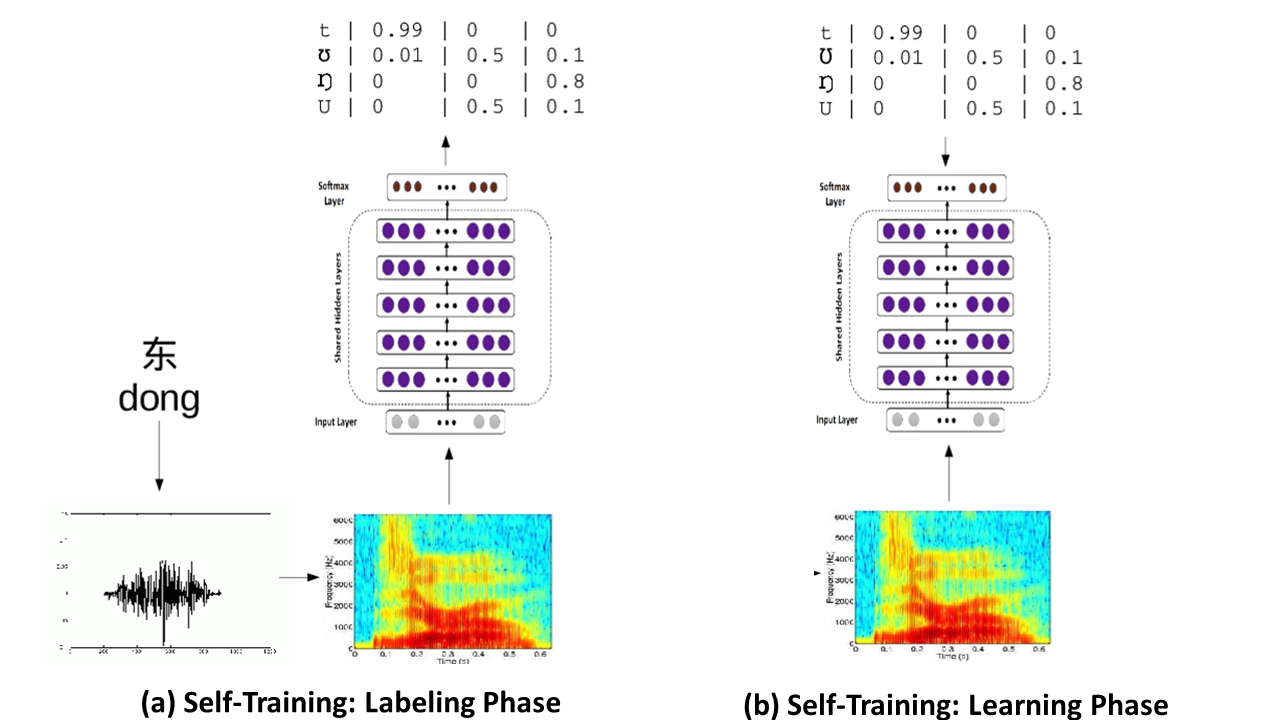
\includegraphics[width=5in]{../figs/fig_hager.png}}
  \caption{The self-training method of~\cite{vesely2013-semi} includes
    a labeling phase and a learning phase.  (a) Labeling phase: an ASR
    trained on other languages (here Cantonese) is used to compute
    posterior phone probabilities $\pi(\phi_t^\ell|x^\ell)$ in the
    test language (here Mandarin). (b) Learning phase: posterior phone
    probabilities are used as targets for DNN re-training.}
  \label{fig:hager}
\end{figure}
%% comments: since the key difference in this figure between the
%% labeling phase and the learning phase is the direction of the upper
%% arrow, I suggest making the arrows more prominent. Also, the text
%% annotating the DNN is illegible, as is the text garnishing the axes
%% of the waveform and spectrograms.

In contrast to the approach in \cite{vesely2013-semi}, which used the
best path alignment as the target in frame cross-entropy training, we
achieved better performance using the posteriors as soft-targets
(Fig.~\ref{fig:hager}). However, we did follow the recommendation in
\cite{vesely2013-semi} to scale the amount of transcribed data by 2 to 
create a good balance between transcribed and untranscribed data.
